\documentclass[12pt]{article}

\title{SCL Example Robot : RPP Bot}      
\author{Samir Menon, smenon@stanford.edu}

\usepackage{graphicx}
\usepackage[top=2cm, bottom=3cm, left=1.5cm, right=1.5cm]{geometry}
%For stretching tables.
\usepackage{tabularx}

\usepackage{amssymb,amsmath}

\begin{document}
\maketitle


\begin{figure}[ht!]
\begin{center}
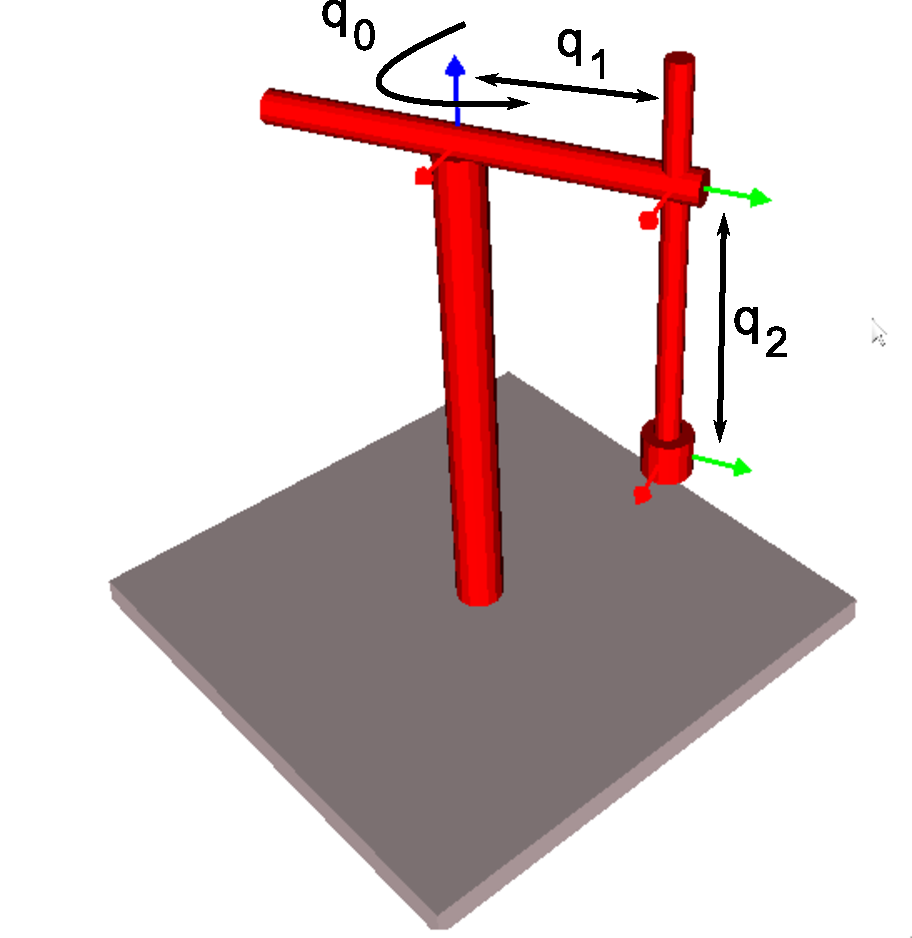
\includegraphics[width=3.5in]{figs/rpp2.pdf}
\caption{RPP Bot Frames: Frame$_0$ rotates with $q_0$ about the z-axis, frame$_1$ moves along the y-axis 
with $q_1$ and frame$_2$ moves along the z-axis with $q_2$. The x, y and z axes are colored red, green 
and blue respectively. Each frame has an offset given in the transformation equations.}
\label{fig:rppframes}
\end{center}
\end{figure}


\section{Description}
RPP is a revolute-prismatic-prismatic robot (Fig. \ref{fig:rppframes}) built to
demonstrate control and dynamics. It is a simple robot whose dynamics can be
computed analytically.

\section{Kinematic Transformations}
The kinematic transformations are useful to transform the motion of a point on the robot
from link-centric coordinates to global coordinates. Trajectories are usually specified in
fixed global coordinates (it is much easier to do so) and a controller can use the kinematics to
compute an error between the position of a point on the robot and the trajectory in global
coordinates.

The robot is connected to a ground frame (-1). Its base frame (frame$_0$) is computed
from the ground frame after a rotation about $q_0$ and a translation up to the
point where link$_0$ connects to link$_1$. Thus, frame$_0$ rotates with link$_0$.
Next, link$_1$ moves along the y-axis, and link$_2$ moves along the z-axis (Fig. \ref{fig:rppframes}).
Offsets for frames 0, 1 and 2 are given by $l_0$, $l_1$ and $l_2$ respectively. 
Frame$_2$ is at the end-effector.

The transformation matrices
\footnote{{\em Notation:} The subscript represents the frame of the vector to be multiplied, 
while the superscript represents the final (transformed) frame.}
 are given by:
\begin{equation}
  ^{-1} T_{0} = 
  \begin{bmatrix} 
  cos(q_0) & -sin(q_0) & 0 & 0 \\ 
  sin(q_0) & cos(q_0) & 0 & 0 \\
  0 & 0 & 1 & l_{0} \\
  0 & 0 & 0 & 1 
  \end{bmatrix}
\end{equation}

\begin{equation}
  ^0 T_{1} = 
  \begin{bmatrix} 
  1 & 1 & 0 & 0 \\ 
  0 & 1 & 0 & q_1+l_{1} \\
  0 & 0 & 1 & 0 \\
  0 & 0 & 0 & 1 
  \end{bmatrix}
\end{equation}

\begin{equation}
  ^1 T_{2} = 
  \begin{bmatrix} 
  1 & 1 & 0 & 0 \\ 
  0 & 1 & 0 & 0 \\
  0 & 0 & 1 & q_2+l_{2} \\
  0 & 0 & 0 & 1 
  \end{bmatrix}
\end{equation}

And any vector may be transformed from the end-effector frame to the ground
frame by the following transformation:

\begin{equation}
  ^{ground-frame} v =  ^{-1} T_0 * ^0 T_1 * ^1 T_2 * ^{end-effector-frame} v
\end{equation}

One may similarly construct the inverse transformations from the ground to the end-effector.

\section{Jacobian}
The Jacobian relates the velocity at the a given cartesian point (the operational point)
 to the velocity of the joints
\footnote{{\em Notation:} A dot on top of any variable represents the time derivative.}.
\begin{equation}
  \dot x = J * \dot q
\end{equation}

For this RPP robot we have:
\begin{equation}
  \begin{bmatrix} 
  \dot x \\
  \dot y \\
  \dot z \\
  \end{bmatrix} 
  = 
  {\Large
  \begin{bmatrix} 
    \frac{\delta x}{\delta q_0} & \frac{\delta x}{\delta q_1} & \frac{\delta x}{\delta q_2} \\
    \\
    \frac{\delta y}{\delta q_0} & \frac{\delta y}{\delta q_1} & \frac{\delta y}{\delta q_2} \\ 
    \\
    \frac{\delta z}{\delta q_0} & \frac{\delta z}{\delta q_1} & \frac{\delta z}{\delta q_2}
  \end{bmatrix} 
  }* 
  \begin{bmatrix}
  \dot q_0 \\
  \dot q_1 \\
  \dot q_2 
  \end{bmatrix} 
\end{equation}

\subsection{Algorithms for Computing the Jacobian}
The Jacobian may be computed in numerous ways using some nifty algorithms. I shall focus
on two of the commonly used ones, and also give you some examples. Note that although both
are useful, it is often easier (but possibly less efficient) to use the geometric method 
because writing out the analytical expression to differentiate is usually tedious.

\subsubsection{Analytical Differentiation: Eg. Computing the Basic Jacobian}
The ``basic Jacobian'', or the Jacobian at the end-effector, is an important special case.
It gives us the change in the end-effector's velocity (in the ground frame 
\footnote{While the task velocities may be specified in any frame, the ground frame is usually
a convenient choice.}) 
for a small change in the joint angles.
For serial robots (like RPP), the end-effector is a natural operational point since 
the robot must move it around to do most tasks and the Jacobian's pseudoinverse translates
task velocities into joint velocities, which can then be controlled by controlling the motors.

We can get the translational velocity Jacobian analytically by taking the gradient of the
end effector expressed in the ground frame. The position\\
\begin{equation}
  ^{ground-frame}pos_{end-effector}
  =
  \begin{bmatrix} x \\ y \\ z \\ \end{bmatrix} 
  = 
  \begin{bmatrix} 
    -(q_1 + l_1) * sin(q_0) \\
    (q_1 + l_1) * cos(q_0) \\
    (l_0+q_2 + l_2)
  \end{bmatrix},
\end{equation}
when partially differentiated with respect to the generalized coordinates gives:
\begin{equation}
  J_v = 
  \begin{bmatrix} 
    -(q_1 + l_1) * cos(q_0) & -sin(q_0) & 0 \\
    \\
    -(q_1 + l_1) * sin(q_0) & cos(q_0) & 0 \\ 
    \\
    0 & 0 & 1
  \end{bmatrix}
\end{equation}

The angular velocity Jacobian is more straightforward. Since translating joints don't
contribute to the angular velocity, this simply sums the contribution of the
rotating joints:
\begin{equation}
  J_\omega = 
  \begin{bmatrix} 
   | \bar{\epsilon} * ^{ground}R_0 \hat{r_0} | ... | \bar{\epsilon} * ^{ground}R_n \hat{r_n} |
  \end{bmatrix},
\end{equation}

{\bf Notation:} $\epsilon$ is zero for revolute joints and one for prismatic joints. 
$\bar{\epsilon} = \neg \epsilon$. Finally, $^0R_i$ is the rotation matrix from 
link$_i$'s frame to the ground frame.

For the RPP, we get:
\begin{equation}
  J_\omega = 
  \begin{bmatrix} 
    0 & 0 & 0 \\
    0 & 0 & 0 \\
    1 & 0 & 0 \\
  \end{bmatrix},
\end{equation}

Combining both, components of the Jacobian gives us the basic Jacobian
\begin{equation}
  J_{ee} = 
  \begin{bmatrix} 
    J_v \\
    J_\omega
  \end{bmatrix},
\end{equation}
which satisfies:
\begin{equation}
  \begin{bmatrix} 
    \dot x \\
    \dot y \\
    \dot z \\
    \omega_x \\
    \omega_y \\
    \omega_z
  \end{bmatrix}_{end-effector}
   = J_{ee}
  \begin{bmatrix} 
    \dot q_0 \\
    \dot q_1 \\
    \dot q_2
  \end{bmatrix}
   =   
  \begin{bmatrix} 
    -(q_1 + l_1) * cos(q_0) & -sin(q_0) & 0 \\
    -(q_1 + l_1) * sin(q_0) & cos(q_0) & 0 \\ 
    0 & 0 & 1 \\
    0 & 0 & 0 \\
    0 & 0 & 0 \\
    1 & 0 & 0 \\
  \end{bmatrix}
  \begin{bmatrix} 
    \dot q_0 \\
    \dot q_1 \\
    \dot q_2
  \end{bmatrix}
\end{equation}


\subsubsection{Geometric Method: Eg. Computing a Center of Mass Jacobian}

Being able to compute various Jacobians is necessary for dynamic operational space control.
One important computation is relating the velocity of the link centers of mass to the 
generalized coordinate velocities, which we shall now do.
\footnote{Doing so allows projecting masses and inertias from cartesian coordinates into
 generalized coordinates. How? Try using the equivalence of kinectic energy in both coordinate
frames to answer the question. Else, read the Dynamics section.}
The method differs from the analytic method in that it doesn't require differentiating
the end-effector position. 

To geometrically compute the Jacobian at a point on a link, we use the fact that a link's 
velocity can only be influenced by joints in the chain from the given link to the ground. Ie.
For the RPP, the revolute joint's velocity influences the prismatic links, but not vice versa.
Next, we compute how each successive joint from the ground to the given link influences its
velocity by using the relation $v = \omega \times r$.

The velocity of the center of mass (com) of the k'th link is then:
\begin{equation}
  \begin{bmatrix}
    v \\
    \omega
  \end{bmatrix}_{com}
  = 
  \begin{bmatrix}
    \sum_{i=0}^{k}
    [ \epsilon_i\, (^{i}R_k\, ^{i}v_{joint}) + 
        \bar{\epsilon_i}\, \omega_{i} \times (^{i}T_k\, ^{i}p_{com})] \\
    \sum_{i=0}^{k}
        \bar{\epsilon_i}\, \omega_{i}
  \end{bmatrix}
\end{equation}

\section{Dynamics}
The robot's dynamics describe the robot's motion characteristics due to its mass and inertia. 
Assuming no external forces (for now), the robot's kinetic energy is given by:
\begin{equation}
  E = \sum_{i=0}^{n-dof} \frac{1}{2} (^{cm}v_i^T * ^{cm} m_i * ^{cm} v_i)
\end{equation}


\section{Operational Space Control}


\end{document}





